\documentclass[xcolor=svgnames]{beamer}
\usecolortheme[named=DarkSlateGrey]{structure}

\usepackage{braket}
\usepackage{amsmath}
\usepackage{feynmp}
\usepackage{graphicx}
\usepackage{listings}
\lstset{language=C++,
  basicstyle=\ttfamily\footnotesize,
  keywordstyle=\color{blue}\ttfamily,
  stringstyle=\color{red}\ttfamily,
  commentstyle=\color{green}\ttfamily,
  morecomment=[l][\color{magenta}]{\#}
  }

\DeclareGraphicsRule{*}{mps}{*}{}
\usetheme{Warsaw}
\setbeamertemplate{footline}[frame number]
\setbeamertemplate{navigation symbols}{}

\title{ROOT}
% A subtitle is optional and this may be deleted
\subtitle{Computer Day Tutorial}

\author{Morgan Askins\\ https://github.com/MorganAskins/root\_tutorial.git}

\date{11 May 2015}

\subject{Physics -- ROOT}

\newcommand{\backupbegin}{
   \newcounter{framenumbervorappendix}
   \setcounter{framenumbervorappendix}{\value{framenumber}}
}
\newcommand{\backupend}{
   \addtocounter{framenumbervorappendix}{-\value{framenumber}}
   \addtocounter{framenumber}{\value{framenumbervorappendix}} 
}


\begin{document}

{\setbeamertemplate{footline}{}
\begin{frame}[noframenumbering]
  \titlepage
\end{frame}
}

%% \begin{frame}{Outline}
%%   \tableofcontents
%% \end{frame}

%%%%%%%%%%%%%%%%%%%%%%%%%%%%%%%%%%%%%
\begin{frame}{ROOT Data Analysis Framework}
  ROOT is a set of data analysis packages, written in C++ at CERN, used mostly in particle
  physics. While the base code itself using some high-level C++ implementation, ROOT itself
  is meant to be useable by novices.
\end{frame}

\begin{frame}{Faces of ROOT}
  Our use of ROOT can be split into 3 different areas
  \begin{enumerate}
  \item ROOT files structures (.root files)
  \item C++ interpreter (CINT and CLING)
  \item Data analysis packages and interaction with .root files
  \end{enumerate}
\end{frame}

\begin{frame}{ROOT Files}
  When taking or simulating data you have freedom to choose how you store that data, whether
  it be proprietary binaries, matlab files, text files, ROOT files, etc.
  \begin{itemize}
  \item ROOT files benefit from being able to directly interact with ROOT analysis packages
  \item They contain a structure that is meaningful in particle physics
  \item They hit a good balance between speed and size.
  \end{itemize}
\end{frame}

\begin{frame}{ROOT File Structure}
  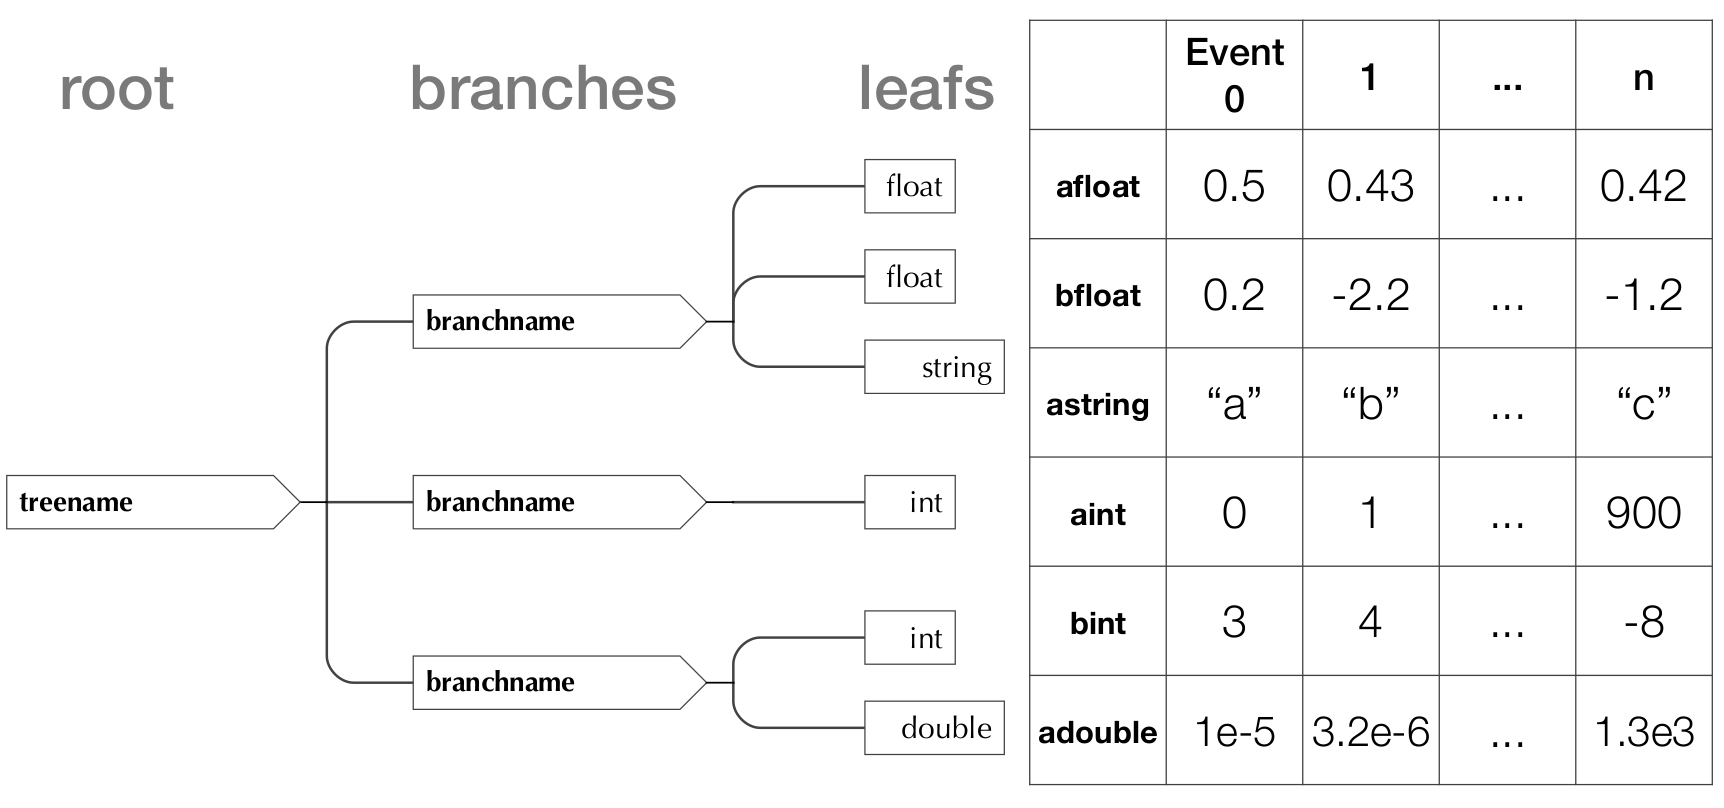
\includegraphics[width=\textwidth]{images/root_structure.png}\\
  \textit{\small Slide Complements Tina Pollmann}
\end{frame}

\begin{frame}[fragile]{Example: Storing data}
ROOT data is stored in a TFile in a directory style format. TFile/TTree/TBranch/TLeaf
\begin{lstlisting}
  #include <TFile.h>
  
  TFile fname("filename.root", "recreate");
  /* Make some Trees, Branches, Histograms etc */
  TTree tree("treename", "tree title");  
  fname.Write();
  fname.Close();
  // And if you prefer writing to heap over stack
  TFile* fname = new TFIle("filename.root", "recreate");
  fname->Write();
  fname->Close();
  delete fname;
\end{lstlisting}
\end{frame}

\begin{frame}[fragile]{Example: Accessing data}
  ROOT data can be accessed in the same way.
  \begin{lstlisting}
    #include <TFile.h>
    
    TFile fname("filename.root", "read");
    /* Now you can access TObjects directly */
    TTree* tree = (TTree*)fname.Get("treename");
    // Make some plots, do some analysis
    fname.Close();
  \end{lstlisting}
\end{frame}

\begin{frame}{C++ Interpreter}
  \begin{columns}
    \begin{column}{0.35\textwidth}
      Advantages of an interpreter
      \begin{itemize}
      \item Prototype code
      \item Explore data structure
      \item Instant analysis
      \item Can load production macros
      \end{itemize}
    \end{column}
    \begin{column}{0.65\textwidth}
      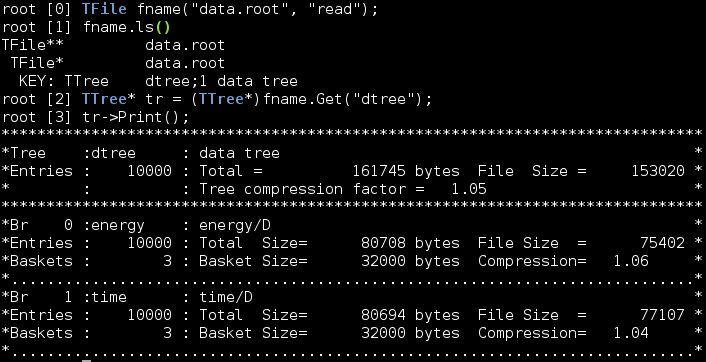
\includegraphics[width=\textwidth]{images/open_tfile.png}
    \end{column}
  \end{columns}
\end{frame}

\begin{frame}{Analysis Tools}
  Most importantly ROOT is used for data analysis.
  Here we create some sample data (see sample\_data.cpp)
  \begin{columns}
    \begin{column}{0.4\textwidth}
      \texttt{tree->Draw("energy");}
      Drawn with TH1F (one dimensional floating point Histogram)
    \end{column}
    \begin{column}{0.6\textwidth}
      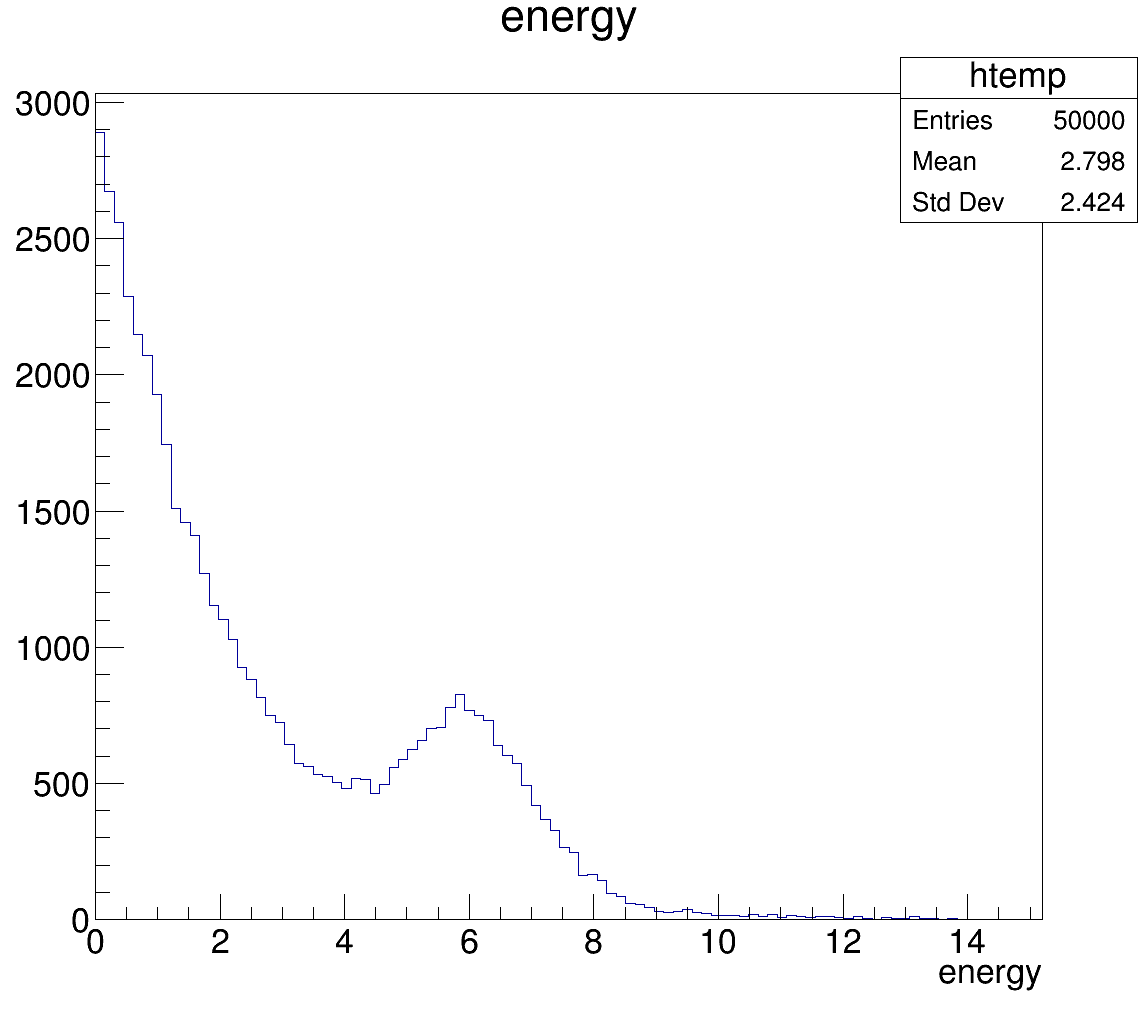
\includegraphics[width=\textwidth]{images/energy.png}            
    \end{column}
  \end{columns}    
\end{frame}

\begin{frame}{Fitting with TF1}
  We can use a TF1 to fit our data: 
  \lstinline{TF1* ff = new TF1("name",}
  \lstinline{ "[0]*TMath::Exp(-x/[1])+[2]*TMath::Gaus(x,[3],[4])", 0, 14)}
  \begin{columns}
    \begin{column}{0.4\textwidth}
      \lstinline{ff->SetParameters(1,1,1,1,1);}
      \lstinline{htemp->Fit(ff);}
      \lstinline{ff->Draw("same");}
    \end{column}
    \begin{column}{0.6\textwidth}
      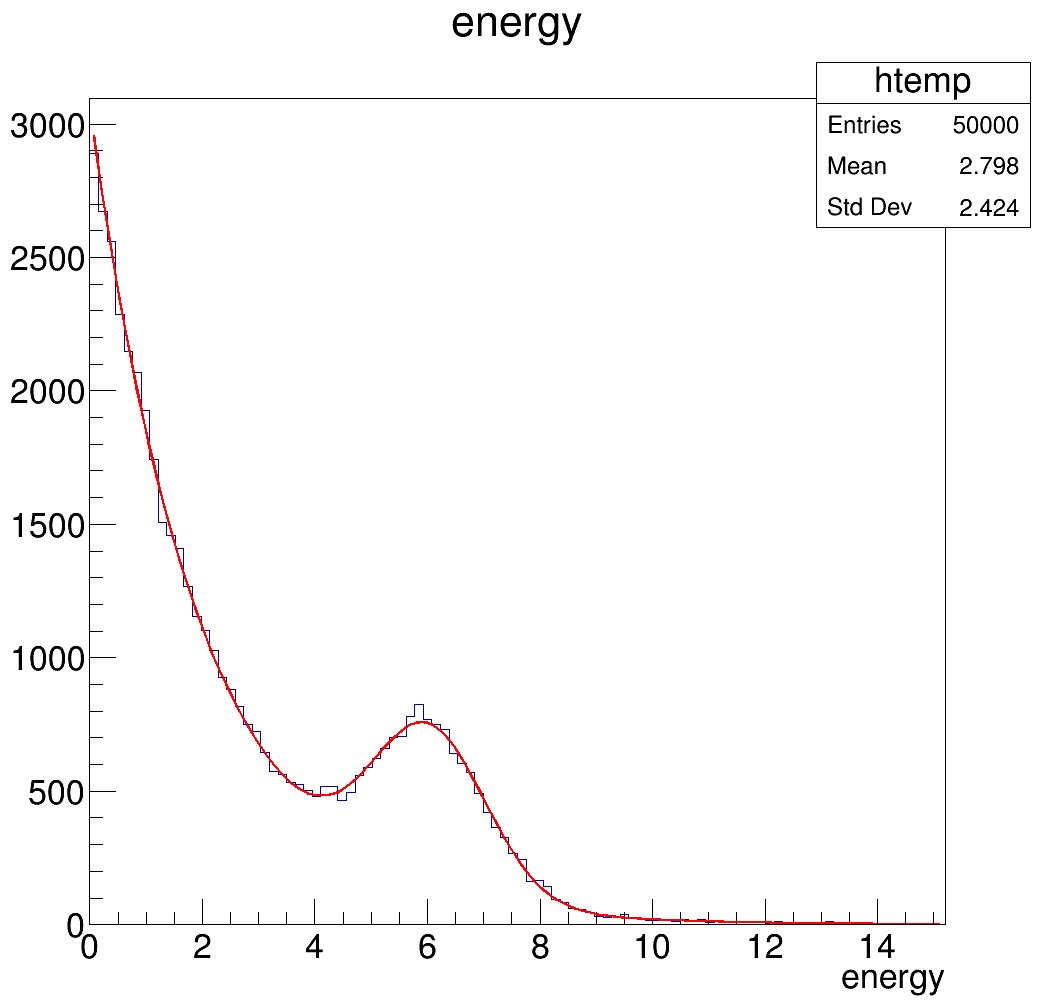
\includegraphics[width=\textwidth]{images/fit.png}
    \end{column}
  \end{columns}      
\end{frame}

\begin{frame}[fragile]{Graphs}
  ROOT can also generate graphs and fit them in the same manner
  \begin{lstlisting}
    double x[5] = {0,1,2,3,4};
    double y[5] = {0,1,4,9,16};
    TGraph gr(5, x, y);
    gr.Draw();
  \end{lstlisting}
  \begin{center}
    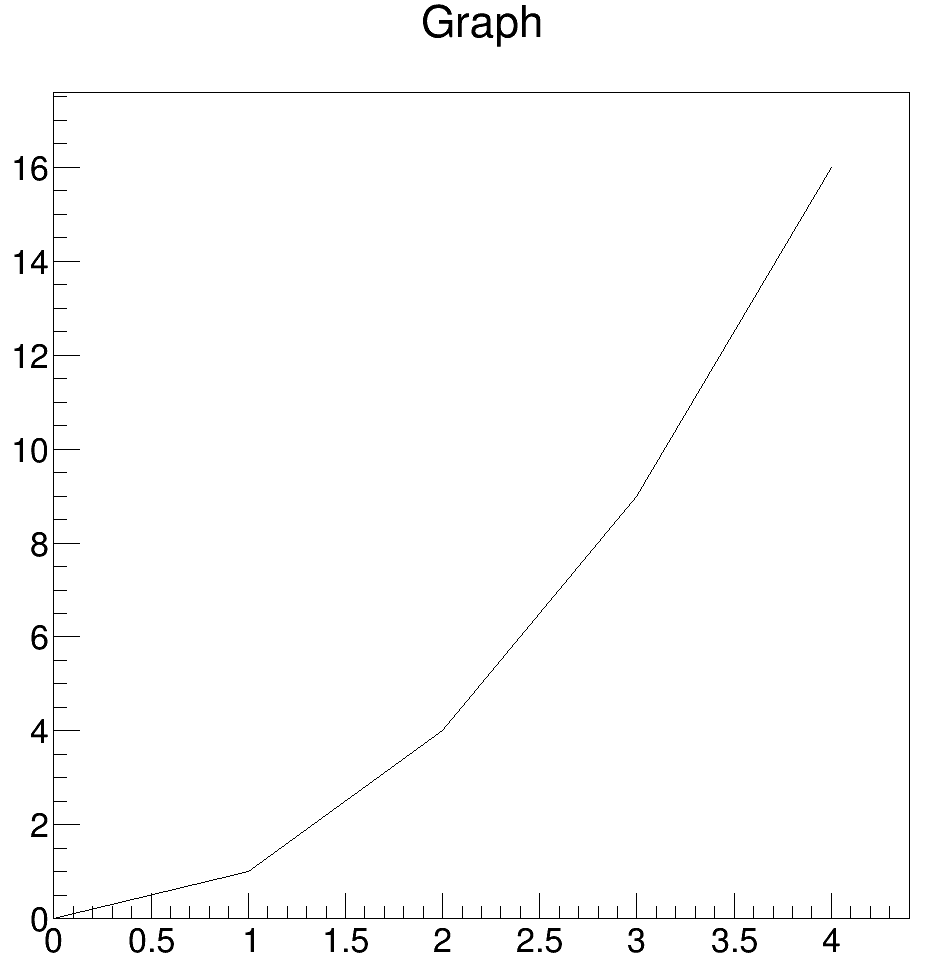
\includegraphics[width=0.5\textwidth]{images/graph.png}
  \end{center}
\end{frame}

\begin{frame}{2D Histograms}
  2D Histograms are also possible (and a lot of fun). See 2d\_data.cpp.\\
  \lstinline{cdata->Draw("two:one", "", "COL");}
  \begin{center}
    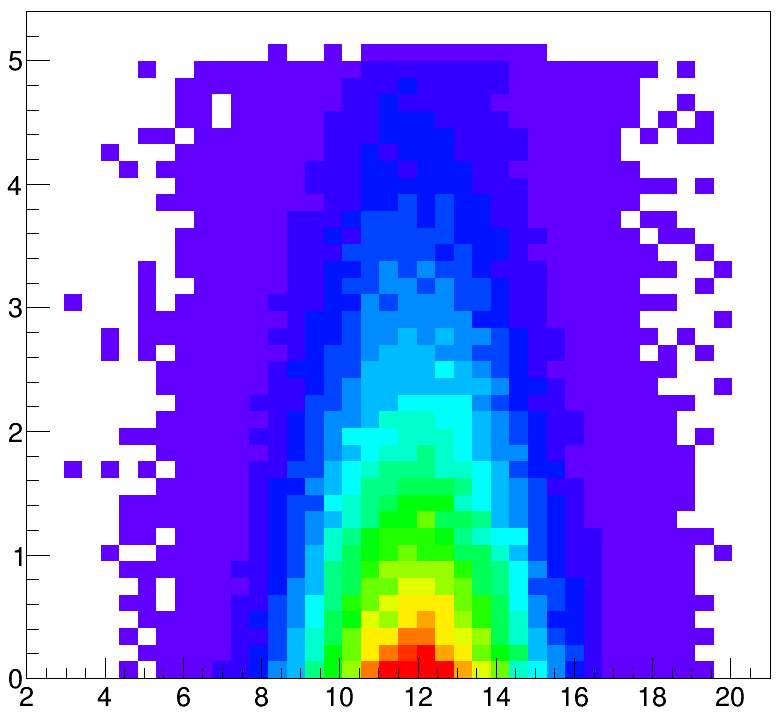
\includegraphics[width=0.6\textwidth]{images/2dhist.png}
  \end{center}
\end{frame}

\begin{frame}[fragile]{TChain}
  Most of the time data will be separated into multiple files. In real data this is split
  into various "runs" depending on configuration, time, and other reasons. In simulation
  one can separate different backgrounds and signals into different files and scale them.
  See chainable.cpp.
  \begin{lstlisting}
    TChain chain("atree");
    chain.Add("tone.root");
    chain.Add("ttwo.root");
    // Could also do chain.Add("t*.root");
    chain.Draw("energy");
  \end{lstlisting}
\end{frame}

\begin{frame}{Running your code}
  \begin{itemize}
  \item Type what you want straight into the interpreter
  \item Write a root macro file and load it into the interpreter (Many ways to do this)\\
    \texttt{root myscript.c} or \texttt{ root [0] .x myscript.c }
  \item Compile with cint ( root -q -b myscript.c )
  \item Compile the code with gcc and run it (See TRint for graphics)\\
    \texttt{g++ `root-config --cflags --glibs` myscript.c }
  \end{itemize}
\end{frame}

\begin{frame}{Excercise 1: Installation}
  The level of difficulty in this task varies greatly depending on operating systems. Here
  is a general guide for installing ROOT.
  \begin{enumerate}
  \item Open a web browser and navigate to google.ca
  \item Type "Install root cern (os name and version)"
  \item Pray your guide simply says
  \end{enumerate}
  Note: The version you want is probably some form of 5.34 (ask your collaboration)
  most collaborations have yet to migrate to 6.xx
\end{frame}

\begin{frame}{Excercise 2: Pretty Plots}
  Given the data from sample\_data.cpp:
  \begin{enumerate}
  \item Fit the data to an exponential + gaussian
  \item Draw both fits separately over data
  \item Plot data with statistical errors
  \item Add a TLegend with data, fit of exp, and fit of gaus
  \item Make a TCanvas with 2 pads and add the same plot on a logscale
  \end{enumerate}
  https://root.cern.ch/root/html534/tutorials/
\end{frame}

%%%%%%%%%%%%%%%%%%%%%%%%
%% BACKUP SLIDES
%%%%%%%%%%%%%%%%%%%%%%%%
%% \backupbegin
%% \begin{frame}{Backup}{Slides}
%% \end{frame}
%% \backupend

\end{document}
